\documentclass[12pt,a4paper]{article}
\usepackage[spanish]{babel}
% \usepackage[utf8]{inputenc}
% \usepackage[dvips]{graphicx}
\usepackage{listings}
\usepackage{graphicx}
\usepackage{afterpage}


\newcommand{\HRule}{\rule{\linewidth}{1mm}}

%\lstset{fancyvrb=true}
\lstset{
	basicstyle=\small,
	tabsize=2,
	numbers=left,
	captionpos=b		
}


\title{Inteligencia Artificial\\ 
\large Informe Final
}
\author{Botta Mariano \\ Campostrini Esteban}
\date{ \small 13 de Septiembre del 2013}

\begin{document}

\maketitle 

\begin{abstract}
El proyecto consiste en dise\~nar y desarrollar un sistema basado en t\'ecnicas de inteligencia artificial capaz de jugar al 
juego de cartas conocido como Truco.
Una descripci\'on completa del juego puede verse en \cite{reglas}. El dise\~no del juego fue pensado para permitir partidas 
entre un humano y una m\'aquina. No se tuvieron en cuenta todas las caracter\'isticas del juego, por ejemplo el canto de ``Flor'' 
no est\'a soportado. El juego puede jugarse on-line entrando a la direcci\'on: http://truco-argento.com.ar

Luego de un an\'alisis del juego optamos por representar la inteligencia artificial mediante un sistema basado en conocimientos, 
m\'as precisamente un sistema experto con reglas de producci\'on de tipo deductivo (Forward Chaining). Si bien no se utiliz\'o un motor
deductivo en particular, los pasos seguidos por el sistema a la hora de tomar las decisiones representan el ciclo b\'asico de un motor deductivo.
\end{abstract}
\pagebreak

\section{Introducci\'on}
El proyecto consiste en el dise\~no e implementaci\'on de un sistema de inteligencia artificial capaz de jugar, de manera realista
una partida de truco contra un oponente humano. Parte de la motivaci\'on que llev\'o a la elecci\'on surgi\'o del hecho de
que es un cl\'asico argentino del que no hay muchas implementaciones disponibles que permitan desafiar la m\'aquina. Entre
estas, se destaca la primera, conocida como TRUCO Arbister \cite{arbister}, nombrada asi en honor a sus creadores (Ariel y Enrique Arbister).\\
La versi\'on que presentamos cuenta con pr\'acticamente todas las caracteristicas o cantos del juego original, siendo la
\'unica excepci\'on el canto de la Flor que por el momento fue dejado afuera. Si bien esto responde a una de las modalidades de 
juego (sin Flor), este canto posiblemente sea a\~nadido en el futuro.
Para la implementaci\'on se eleigi\'o JavaScript y HTML haciendo de esta manera posible su ejecuci\'on desde diferentes plataformas. 


\section{Lenguaje y Desarollo}
\subsection{Sobre el lenguaje usado}
El lenguaje en el que se escribi\'o el juego es JavaScript. Si bien durante el cursado de la materia se vieron motores de reglas 
apropiados para modelar este tipo de sistemas (como JESS por ejemplo) no encontramos un recurso de este tipo que estuviese enfocado
al desarrollo de aplicaciones web. Como una de las metas que te\'iamos en realaci\'on a la implementaci\'on era aprovechar la ``generalidad'' que
provee una p\'agina web para hacer una aplicaci\'on multiplataforma, decidimos continuar y modelar la toma de decisiones de 
una manera que respeta, a nuestro entender, la filosof\'ia de un motor de reglas.

\subsection{Breve descripcion de la arquitectura}
El juego junto con la inteligencia artificial fueron desarrollados desde cero en una interfaz web. 

La interfaz gr\'afica esta hecha con HTML y CSS. La l\'ogica del juego est\'a escrita en Javascript y est\'a separada en 2 modulos principales.  
\begin{itemize}
\item El modulo \textbf{truco.js} provee las estructuras de datos necesarias para la representacion de la informacion utilizada durante el juego,
controla la interacci\'on entre el jugador y la m\'aquina, es decir, determina quien puede jugar en un momento determinado y lleva cuenta del
estado global del juego.

\item El modulo \textbf{ia.js} continene la inteligencia artificial de la m\'aquina. Aqu\'i se encuentra codificado el razonamiento realizado por la maquina
a la hora de tomar una decisi\'on.

\end{itemize}

A modo de dar una visi\'on general, el sistema funciona de la siguiente manera: \\
Si el usuario es mano, cualquier acci\'on que ejecute ser\'a procesada por el modulo \textbf{truco.js}. Este se encargar\'a de contextualizar la
acci\'on (por ejemplo, determinar en que mano se realiz\'o el canto y/o si hubo un canto anterior a ese) y llamar\'a al correspondiente m\'etodo del
m\'odulo \textbf{ia.js} que usando esta informaci\'on como conocimiento de dominio, determinar\'a con qu\'e acci\'on responder.



\section{Conocimiento de Dominio}

\subsection{Sobre el enga\~no en el truco}

El truco es un tipo de juego con informaci\'on parcial en el sentido en que al menos uno de los jugadores
conoce solo un estado parcial del juego (en caso de un desarrollo ``normal'' del juego, esto deber\'ia 
pasar para todos los jugadores involucrados). Esto implica una complejidad mayor a la hora de tomar decisiones
ya que es necesario tener en cuenta las jugadas pasadas como las posibles jugadas futuras. 
El hecho de que cada jugador ignore una parcialidad del estado del resto de los oponentes puede ser aprovechado
de manera ``maliciosa'' por parte de alguno de ellos para intentar inducir estados falsos que den lugar a que otro jugador
tome una mala decisi\'on de juego. En el truco este enga\~no puede manifestarse de dos formas (que osamos en llamar
activa y pasiva)\\
\textbf{Activa:} el jugador toma la iniciativa mediante alg\'un canto (envido o truco) con el fin de hacerle creer al oponente que tiene
cartas o puntos que en \\ realidad no tiene.\\
\textbf{Pasiva:} el jugador plantea un escenario (generalmente mediante el orden en el que juega las cartas) de manera tal de que 
la hipotetizaci\'on hecha por el oponente sobre el estado sea err\'onea llev\'andolo a tomar acciones 'activas' poco favorables para 
\'este (b\'asicamente que el jugador que est\'a intentando ser enga\~nado piense que el otro jugador tiene m\'as o menos puntos o cartas de 
mayor o menor valor que en las que realidad tiene).\\
Cabe destacar que un intento de enga\~no tanto activo como pasivo est\'a influenciado tambi\'en por la informaci\'on que uno tiene del otro jugador,
que en la mayoria de los casos sigue siendo parcial,  por lo cual hay una especie de circulo de mentiras.\\
De aqu\'i, que el enga\~no juega un rol importante en el truco.

\subsection{Funciones principales}
El c\'odigo del juego est\'a disponible en \cite{codigo}
Como se explica en la secci\'on anterior, el enga\~no es parte del juego y este est\'a generalmente influenciado por
la informaci\'on disponible, lo cual tambi\'en implica que no hay una estrategia ganadora. 
A continuaci\'on haremos una descripci\'on de las funciones principales de la Inteligencia Artificial comentando c\'omo fue tenida en cuenta la 
informaci\'on disponible y de qu\'e manera se intent\'o darle ``picard\'ia'' al programa.

%Este juego es muy particular, no existe una f\'ormula ganadora. Depende mucho de la picard\'ia del jugador. Por eso, apesar de estar basado en un sistema experto
%con reglas, en muchos cosas como \'ultima opci\'on se agrego un poco de no-determinismo para crear una sensaci\'on  de que no es una maquin\'a est\'atica. 
%Este no determinismo esta fuertemente influenciado por el conocimiento de dominio.

Luego de analizar la metodolog\'ia de juego, se opt\'o por dividir el dise\~no del programa en 3 partes diferentes:
\begin{itemize}
\item Truco: se encarga de decidir los cantos del truco
\item Envido: decide el canto del envido
\item Jugar Carta: decide que carta jugar
\end{itemize}
 

\subsubsection{Truco}
%La informaci\'on que consideramos pertinente a la hora de decidir el canto del truco esta
%representada por las siguientes variables:
Esta es la informaci\'on que consideramos pertinente a la hora de decidir el canto del truco:
\begin{itemize}
\item Informaci\'on sobre si el humano cant\'o algo y la m\'aquina debe contestar o si esta puede cantar (variable \textbf{resp})
%\item resp: valor booleano que indica si el humano cantó algo y por lo tanto la m\'aquina tiene que contestar o si esta puede cantar.
\item El \'ultimo canto hasta el momento en la ronda actual (variable \textbf{ultimo})
\item El n\'umero de la mano actual (primera, segunda o tercera)
\item Resultado de las manos anteriores
\item Cartas jugadas en la mano actual (propias o del oponente)
\item Clasificaci\'on de las cartas en mano (cantidad de cartas altas, medias o bajas que tengo).
\item Posibles cartas del oponente seg\'un los puntos cantados en el envido y las cartas que jug\'o.
\end{itemize}

Mediante todos estos atributos se conforman las reglas de inferencia que se dividen, de manera general, de la 
siguiente forma:

\begin{itemize}
\item 1) Contestar un canto o Cantar
\item 2) Se determina cual es la mano actual
\item 3) Se determina el resultado de la mano anterior (para las manos 2 y 3)
\item 4) Se clasifican las cartas que poseo
\item 5) En funci\'on de la situaci\'on en la que se encuentre y teniendo en cuenta los datos correspondientes al dominio
	   se decide que cantar (Si, No, Re-Truco, Vale 4)
\end{itemize}

Veamos un extracto del c\'odigo de la funci\'on truco a modo ilustrativo:
\begin{figure}[h]
\lstset{language=java,caption=Extracto de la funci\'on truco,label=lst:nicecode}
\begin{lstlisting}

if (resp) {  // Me cantaron, tengo que responder
	switch(nroMano){
		case 0:
			var ran = getRandomInt(0,100);
			switch(ultimo){
		case 'T':
			if (e2.jugador.puntosGanadosEnvido < 2 && 
					(mediaalta) >= 2 && clasif.alta >= 1)
				return 'S';
			if (clasif.baja === 3 && ran <= 50) return 'RT'; 
			if (mediaalta >= 2 && diff < 0  ) return 'RT';  // Te trato de correr
			if (mediaalta >= 1 && diff > 0  ) return 'S';
			return ( ran < 66 ? 'N' : 'S' ); //  (*) Rompe con la reglas staticas
		case 'RT':
		case 'V':
			if (clasif.alta >= 2) return 'S';
			if ((mediaalta) >= 2  && diff > 3 ) return 'S';
			if (e2.jugador.puntosGanadosEnvido >= 2) return 'N';
			return 'N';
			break;
		}
	}
}
\end{lstlisting}
\end{figure}


\noindent En este caso vemos qu\'e sucede cuando el oponente canta algo (la variable \textbf{resp} toma el valor true). Primero determinamos
en que n\'umero de mano nos encontramos. Luego en funci\'on de lo que fue cantado por el oponente (truco - T, re-truco - RT, o vale 4 - V)
y en funci\'on de las cartas en mano as\'i como de los puntos obtenidos en el envido se decide que acci\'on tomar. Se puede ver tambi\'en
una componente aleatoria. Si bien no es un recurso ideal, nos encontramos con el hecho de que una vez colectada toda la informaci\'on posible
(que es incompleta) siempre hay un factor no determinista (simpre hay m\'as de un camino a seguir)
que podr\'ia ser ignorado poniendo reglas fijas pero esto har\'ia que el comportamiento de la m\'aquina sea bastante ``r\'igido''.

\subsubsection{Envido}
%El conocimiento de dominio que utiliza comprende:
La informaci\'on tenida en cuenta comprende:
\begin{itemize}
\item El \'ultimo canto realizado (variable \textbf{ultimo})
\item La cantidad de puntos en juego (variable \textbf{acumulado})
\item Carta jugada por el oponente (si es que existe) y deducci\'on de posibles puntos (variable \textbf{ultimaCarta})
\item Puntos de Envido en mano (variable \textbf{puntos})
\item Puntos restantes para terminar el partido
\item Puntos con lo que el oponente canto en otras manos
\item Puntos que se pierden si no se acepta el envido (variable \textbf{puntosNoQuerido})
\end{itemize}


Para decidir el canto del envidio, primero se analiza los puntos restantes para terminar la partida debido a que la Falta Envido es diferente al 
resto de los cantos. Si faltan dos o menos puntos para ganar, se responde a cualquier canto de envido cantando la Falta. De igual manera, dadas
las mismas condiciones si no se cant\'o nada y es el turno de la m\'aquina, se canta la Falta.\\
\noindent En caso de estar a mediados del juego se tiene en cuenta si hubo cantos previos, si el oponente ya jug\'o una carta y la cantidad de puntos que tengo en mano. 
Todos estos valores generan una decisi\'on de juego, a la que en \'ultima instancia se le agrega un factor aleatorio, con el fin de evitar nuevamente
un comportamiento fijo en la m\'aquina.

%\newpage


\begin{figure}[h]
\lstset{language=java,caption=Extracto de la funci\'on envido,label=lst:nicecode}
\begin{lstlisting}
switch(ultimo){
	case 'E':
		var pRE = this.prob.promedioPuntos(this.envidoS)  ;
		pRE =  pRE === null ? 0 :  pRE - 15 ; 
										                  
		if (ran + posible + diff + acumulado + pRE  <  valor  * 100 ) {
			if (puntos >= 30 ) return  'EE' ; 
			else return 'S';
		} 
		else { 
			if (puntos >= 30 ) return 'S'; 
			else  return 'N';  
		}
		break;
}

\end{lstlisting}
\end{figure}

\noindent En el extracto anterior se puede ver como se procesa el caso en el que el humano canta Envido.
La variable \textbf{pRE} se inicializa con el promedio del historial de puntos con los que el humano
cant\'o envido hasta ese momento. En la siguiente l\'inea se hace un corrimiento, centrando en cero el valor
(tomando 15 como la mitad de los puntos que uno puede tener en el envido). La idea es que si el humano
solia cantar hasta ese momento con menos de 15 puntos, el valor de pRE va a ser negativo y va a contribuir
a que el primer if evalue a verdadero, dando lugar a que la m\'aquina revire (en terminos m\'as familiares,
si el oponente suele cantar con pocos puntos, despu\'es de un tiempo va a perder algo de credibilidad y voy 
a considerar revirarle en alg\'un momento).\\
\noindent En el If siguiente se puede ver la expresi\'on: 
\begin{center}
	$ ran + posible + diff + acumulado + pRE  <  valor  * 100 $
\end{center}
que representa el recurso que usamos para introducir no determinismo. La idea es tener en cuenta a la hora de revirar
o aceptar el envido, las variables que uno analizar\'ia en un juego normal, ante otras personas. B\'asicamente son 
(est\'an tambi\'en explicadas m\'as arriba): qu\'e es lo que puede tener el oponente, cu\'al es la diferencia de puntos
en el partido entre el oponente y yo, cuantos puntos hay en juego en este momento y el historial de canto del oponente.\\
\noindent A esto le agregamos una componente aleatoria como valor final a tener en cuenta.
Como ya mencionamos, los jugadores siempre tienen informaci\'on parcial o incompleta, lo que imposibilita
determinar la elecci\'on \'optima y da lugar al no-determinismo. Es por esto que se induce un sesgo o arbitrariedad
a la hora de tomar la decisi\'on, que creemos no es completamente artificial (no es de extra\~narse que durante una partida entre
2 humanos surjan en m\'as de una ocasi\'on situaciones como esta que terminan siendo resueltas por arbitrariedades, algunas de
ellas basadas en caracteristicas inherentes a una persona como gestos faciales o modulaci\'on de la voz, pero arbitrariedades
al fin). 
La componente aleatoria es comparada con un valor que asignamos a los puntos que tenemos en mano. 
Los valores a ambos lados de la desigualdad est\'an entre 0 y 100.
%% Revisar estooo ultimo!!!! 



\subsubsection{Jugar Carta}
El conocimiento de dominio que utiliza comprende:
\begin{itemize}
\item Juego primero o  el oponente ya jugo
\item Clasificaci\'on de las cartas
\item Numero de Mano
\item Carta jugada por el oponente
\end{itemize}

Para determinar que carta jugar primero se tiene en cuenta si el oponente jugo. Si es as\'i elige la carta en 
funci\'on de la que esta en la mesa. Depende de si le puede ganar o no.
Si la m\'aquina es mano, por lo general opta por la siguiente f\'ormula: Ganar primera, dejar pasar segunda y ganar tercera. 
Por supuesto hay reglas , que capturan situaciones especiales, provocando una variaci\'on al juego de la m\'aquina. Por ejemplo, si es mano y posee dos cartas altas.


El conocimiento de dominio necesario fue aportado por los integrantes del grupo 

\section{Resultados y conclusiones}
Luego de varias partidas llevadas a cabo por voluntarios gentilmente ofrecidos asi como por nosotros,
podemos decir que el comportamiento del programa se asemeja razonablemente al de un humano no-experto. 
Sin duda, si una persona se sienta con una libreta y juega lo sufuciente, tomando nota de los distintos escenarios y las
distintas respuestas del programa, pueden quedar expuestos patrones que permitan determinar una gran parte
,o quiz\'a la totalidad, del conjunto de reglas que conforman la inteligencia artificial. Esto es algo
que puede hacerse con m\'as de un juego y que sin poder evitarlo, intentamos que sea lo m\'as dif\'icil
posible de hacer. \\
Con respecto a la implementaci\'on, llegamos a la conclusi\'on de que es un juego que cuenta con un 
gran nivel de no determinismo que dificulta su modelado mediante el uso de reglas. El hecho
de que se cuenta solo con informaci\'on parcial da lugar que en ciertos momentos sea imposible determinar 
cual es la jugada \'optima.
De todas maneras la bater\'ia de reglas que componen la inteligencia artificial puede ser extendida de 
manera incremental haciendo que la granularidad en los detalles tenidos en cuenta por el programa
a la hora de tomar una decisi\'on sea mayor, obteniendo asi un comportamiento m\'as complejo 
y ``real''.

\section{Capturas de pantalla}
Las siguientes capturas de pantalla grafican distintas etapas del juego.

\clearpage
\begin{figure}
\begin{center}
\noindent \makebox[\textwidth] {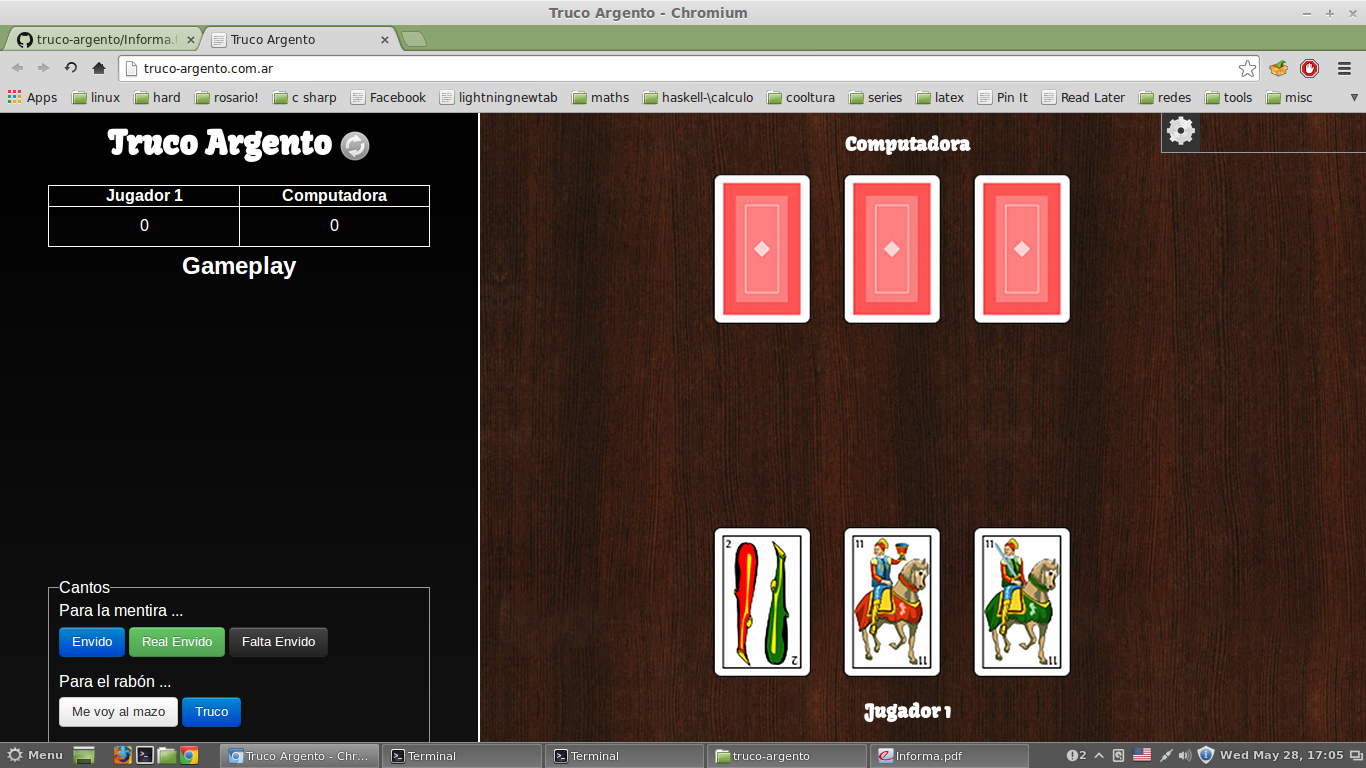
\includegraphics[width=\linewidth]{truco1.png}}
\caption{Comienzo del juego.}
\end{center}
\end{figure}

\begin{figure}
\noindent \makebox[\textwidth]{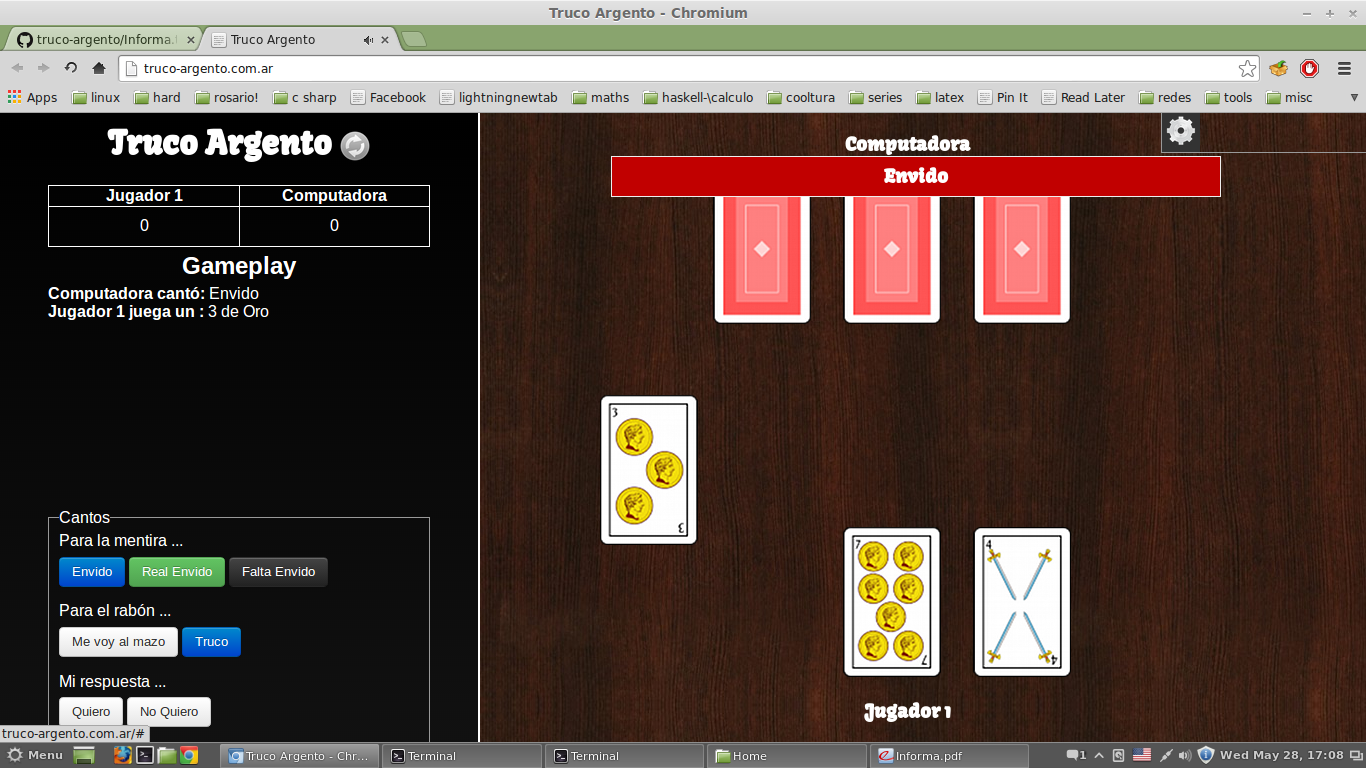
\includegraphics[width=\linewidth]{envido1.png}}
\caption{El programa canta envido.}
\end{figure}

\begin{figure}
\noindent \makebox[\textwidth]{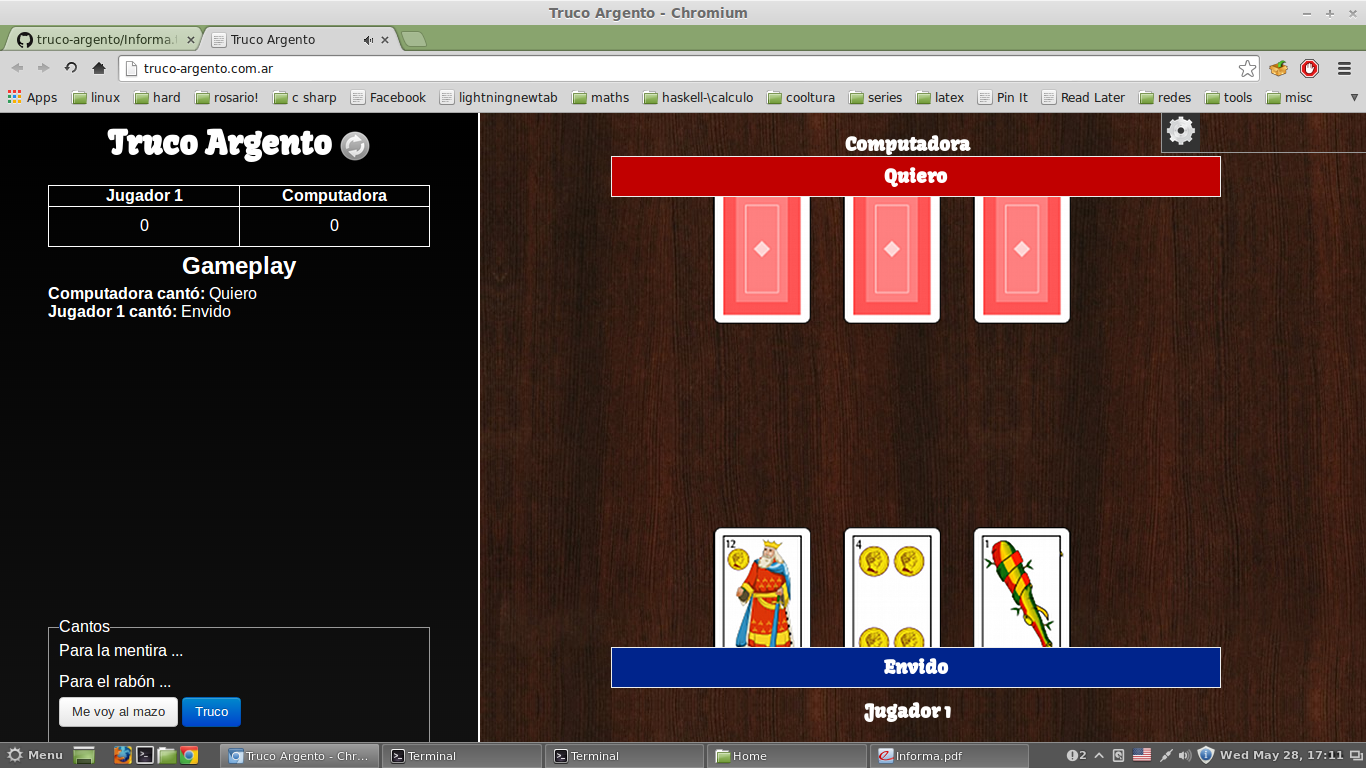
\includegraphics[width=\linewidth]{envido2.png}}
\caption {El humano canta envido y el programa acepta.}
\end{figure}

\begin{figure}
\noindent \makebox[\textwidth]{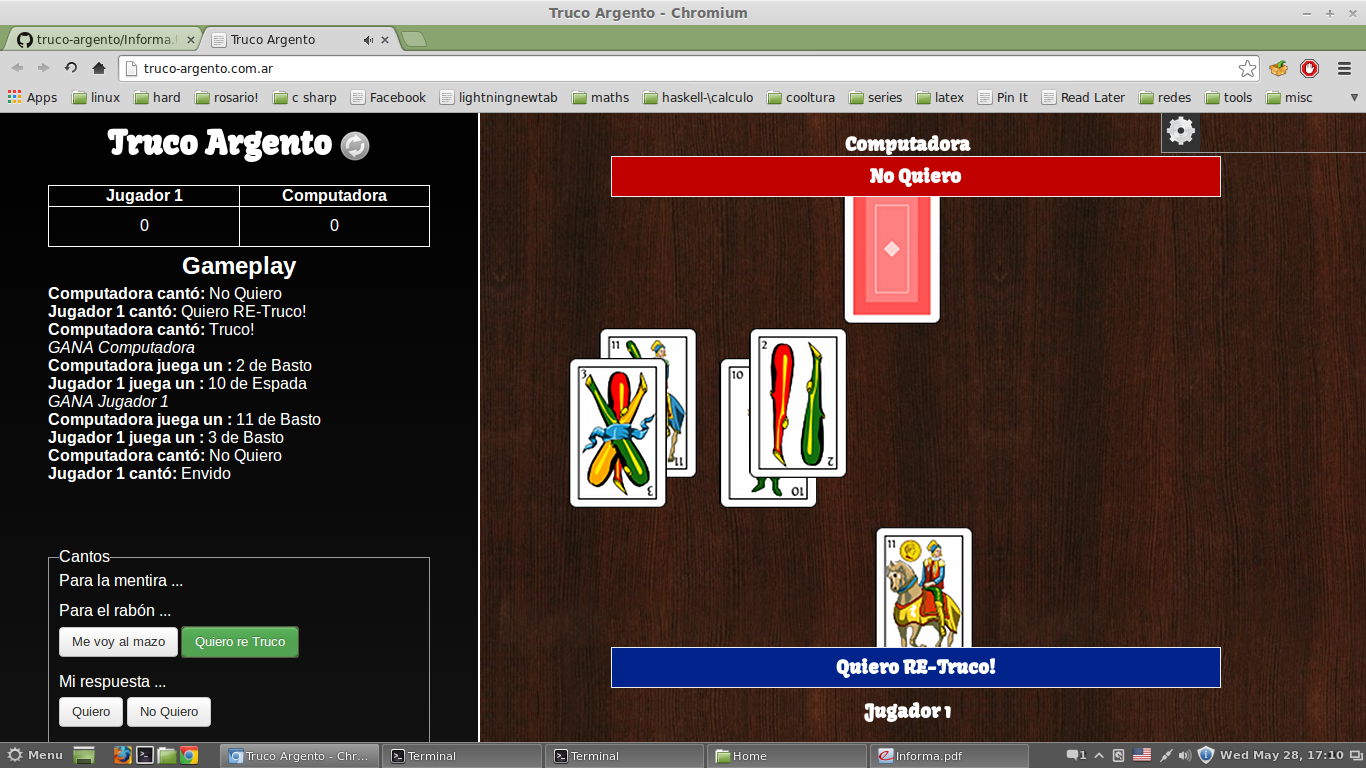
\includegraphics[width=\linewidth]{retruco.png}}
\caption {El humano retruca y el programa no acepta.}
\end{figure}

\clearpage
\begin{thebibliography}{9}

	\bibitem{reglas} \emph{Descripci\'on y Reglas del Truco }. 
	http://es.wikipedia.org/wiki/Truco\_argentino .

	\bibitem{arbister} \emph{Primer truco interactivo }. 
	http://www-2.dc.uba.ar/charlas/lud/truco .

	\bibitem{codigo} \emph{C\'odigo del juego}.
	https://github.com/p4bl1t0/truco-argento.git



\end{thebibliography}
\end{document}

